%!TEX root = volumeFinal.tex 
\chapter{\label{chap:planejamento}Planejamento automatizado}

Planejamento automatizado é uma sub-área da inteligencia artificial que estuda o processo de geração automática de planos. O processo para gerar um plano, é feito a partir da escolha e organização das ações, antecipando os resultados esperados das ações, em busca do seu objetivo. Um plano pode ser descrito como uma sequencia de ações que se forem executadas chegam a um objetivo \cite{ghallab2004automated}. O planejamento na computação se diferencia das outras áreas pelo fato de que todo o plano é gerado automaticamente \cite{intelligence2003modern}. 

\section{Representação do problema}
Uma entrada para qualquer técnica de planejamento é uma descrição do problema a ser resolvido. Isso é necessário para não precisar representar todos os estados e transição do problema. Com a descrição do problema os estados e transição não precisam ser explícitos, mas faz com que os estados não descritos possam ser computados \cite{ghallab2004automated}. Como foi visto no capitulo \ref{chap:agentes}, os estados são os estados para o agente se situar no ambiente e transições são para a interação com o ambiente. Um problema de planejamento pode ser descrito como \textit{P} = \textit{($\Sigma$, $s_{0}$, g)}. Onde \cite{ghallab2004automated}:

\begin{itemize}
	\item $\Sigma$- é a representação do problema;
	\item $s_{0}$- é o estado inicial, estado onde o problema começa;
	\item g- é o objetivo, estado onde o problema deve acabar.
\end{itemize}

Para representar o problema é necessário representar os estados do ambiente. Uma forma de fazer isso é utilizando lógica matemática. Sendo assim um estado do ambiente é representados por um conjunto de átomos que resultam em verdadeiro ou falso dependendo da interpretação do ambiente \cite{ghallab2004automated}. Vamos lembrar do problema do Capitulo \ref{chap:busca}, chegar a uma determinada cidade, estados para esse problema podem ser estar em determinada cidade e ter ligação entre as cidades, representado respectivamente como \textit{estar(cidade)} \textit{terLigação(cidadeOrigem, cidadeDestino)}.   

Além dos estados do ambiente precisamos determinar as transições, que alteram os estados. As transições utilizam ações e são representadas por operadores de planejamento que alteram os valores dos átomos presentes em determinado estado. Um operador de planejamento é definido como \textit{op} = (nome(\textit{op}), precondições(\textit{op}), efeitos(\textit{op})), onde cada elemento é definido como \cite{ghallab2004automated}: 

\begin{itemize}
	\item nome(\textit{op}) - É o nome do operador de planejamento e \textit{op} é o conjunto de todas as variáveis que irão aparecer qualquer parte do operador de planejamento.  
	\item precondições(\textit{op}) - \textit{op} é o conjunto de átomos ou átomos negativos que representa a precondição do operador de planejamento. 
	\item efeitos(\textit{op}) - \textit{op} é o conjunto de átomos ou átomos negativos que representa o efeito do operador de planejamento
\end{itemize}

No nosso exemplo, um operador de planejamento seria a mudança de uma cidade A para outra cidade B, que poderia ser representado como:
\begin{itemize}
	\item nome- mudarDeCidade(cidadeA, cidadeB);
	\item precondições- estar(cidadeA) $\wedge$ terLigação(cidadeA, cidadeB);
	\item efeitos- $\neg$ estar(cidadeA) \and estar(cidadeB).
\end{itemize}  

O nome deve ser único pelo proposito de o nome poder se referir ao operador por completo, ou seja, após definido apenas com o nome pode-se inferir as pré e pós condições, assim escrevendo o nome(\textit{op}) para se referir a todo o operador de planejamento \textit{op} \cite{ghallab2004automated}. 

O processo de geração do plano é feito pelo planejador, para isso ele utiliza a representação do problema, o estado inicial e os objetivos como entrada \cite{ghallab2004automated}. A figura \ref{fig:planmodelo} representa esse processo. 

\begin{figure}[ht]
	\centering
	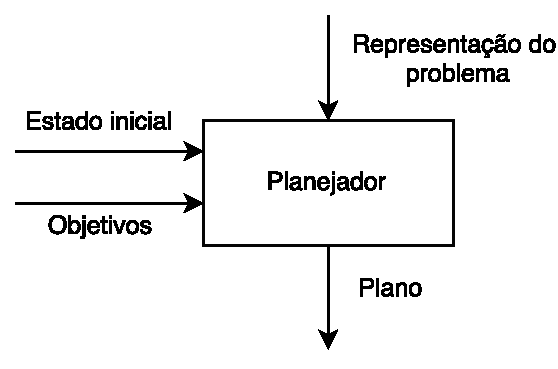
\includegraphics[width=0.4\textwidth]{fig/modelo.pdf}
	\caption{Problema de planejamento}
	\label{fig:planmodelo}
\end{figure} 

O domínio do problema é a parte do mundo que é expressada pelo conjunto de informações que é usado pelo planejador para gerar o plano \cite{intelligence2003modern}. No nosso exemplo, se representássemos as cidades presentes no mapa, apenas aquelas cidades seriam nosso domínio, e a única ação disponível no domínio seria mudar de cidade.

%\msr[inline]{Falar mais de domínio? exemplos de domínios?}

\section{HTN} 

Dentro da área de planejamento existe o planejamento hierárquico, chamado de \textit{Hierarchical Task Network} (HTN). Em planejamento HTN as ações são tratadas em mais alto nível \cite{intelligence2003modern}. Essa abordagem de planejamento cria planos decompondo tarefas em tarefas ainda menores \cite{ontanon2015adversarial}.

Uma tarefa $t$ é uma representação de uma atividade no ambiente. Existem dois tipos de tarefa \cite{intelligence2003modern}: 

\begin{itemize}
	\item Tarefas primitivas- Uma atividade que um agente possa executar diretamente no ambiente.
	\item Tarefas não-primitivas- Representa objetivos que o agente deve alcançar antes que ele possa executar-las, ou seja, tarefas que devem ser decompostas em tarefas menores até todas serem tarefas primitivas. 
\end{itemize}

Para decompor as tarefas não-primitivas em primitivas é necessário um conjunto de métodos \cite{ghallab2004automated}. Um método é composto por $m = (t, C, w)$. Um método m representa uma maneira na qual pode-se decompor as tarefas $t$ em um conjunto de sub-tarefas $w$ se todas as pre-condições C forem satisfeitas \cite{ontanon2015adversarial}.

O planejamento HTN $N$ é feito decompondo tarefas não primitivas recursivamente até chegar em tarefas primitivas \cite{ghallab2004automated}. $N$ é uma arvore, na qual os nodos são tarefas ou métodos. Cada tarefa não-primitiva pode ter apenas um filho, que deve ser um método. Um método tem um filho para cada uma das tarefas em $w$. Tarefas primitivas não podem ter filhos. Uma arvore totalmente decomposta, é onde todas as folhas de $N$ são tarefas primitivas \cite{ontanon2015adversarial}.

Um problema de planejamento HTN pode ser descrito como, $ P = (S, A, \gamma, T, M, s_{0}, N_{0}) $. S é o conjunto dos possíveis estados do ambiente. A é o cojunto finitio das ações que podem ser executadas pelo agente. $\gamma$ é a função de transição que define os efeitos de cada ação no ambiente. T é o cojunto de tarefas. M é o conjunto de métodos. $s_{0} \in S$ é o estado inicial do agente. $n_{0}$ é estado inicial do ambiente, que servem para definir os objetivos do agente. O proposito do planejamento HTN é achar uma arvore N totalmente decomposta que tenha como estado inicial da arvore $n_{0}$ e estado inicial do agente $s_{0}$ \cite{ontanon2015adversarial}.

A ideia do planejamento HTN é através desta descrição do problema de planejamento HTN, decompor o estado inicial e continuar decompondo as tarefas que restarem pelo conjunto de métodos, até só restarem tarefas primitivas. O plano é composto apenas por tarefas primitivas. Na busca pelo plano, o planejamento HTN começa planejando por um caminho, quando um caminho de resolução leva a um fim de linha é realizado um retrocesso(\textit{backtracking}) até um caminho que tenha uma possibilidade diferente de caminho do que foi tomado anteriormente \cite{intelligence2003modern}. 

\section{AHTN} 

\textit{Adversarial hierarchical-task network} (AHTN) é um algoritmo proposto para tentar solucionar o problema do grande fator de ramificação dos jogos em tempo real \cite{ontanon2015adversarial}. Nele são combinados técnicas de HTN com o algoritmo \textit{minimax search}. O algoritmo assume jogos totalmente observáveis, baseados em turno e determinísticos.

O algoritmo \ref{alg:ahtn} \cite{ontanon2015adversarial} é a representação da técnica de AHTN, e assume que existem dois jogadores, MAX e MIN, como no algoritmo de \textit{minimax search} apresentado no capitulo \ref{chap:busca}. O algoritmo também assume uma busca em uma arvore com uma máxima profundidade $d$.

\begin{algorithm}
	\caption{AHTN}
	\label{alg:ahtn}
	\begin{algorithmic}[1]		
		\Function {AHTNMax}{$s, N_{+}, N_{-}, t_{+}, t_{-}, d$}
		\If {$terminal(s) \vee d \leq 0$}
		\State	\Return $(N_{+}, N_{-}, e(s))$
		\EndIf
		\If {$nextAction(N_{+}, t_{+}) \neq \perp$}
		\State $t = nextAction(N_{+}, t_{+})$ 
		\State \Return $AHTNMin(\gamma(s,t), N_{+}, N_{-}, t, t_{-}, d-1)$
		\EndIf
		\State $N_{+}^{*} = \perp, N_{-}^{*} = \perp, v^{*} = -\infty$
		\State $\aleph = decompositions_{+}(s, N_{+}, N_{-}, t_{+}, t_{-})$
		\ForAll{$N \in \aleph$}
		\State $(N^{'}_{+}, N^{'}_{-}, v^{'}) = AHTNMax(s, N, N_{-}, t_{+}, t_{-}, d)$
		\If{$v^{'} > v^{*}$}
		\State $N_{+}^{*} = N^{'}_{+}, N_{-}^{*} = N^{'}_{-}, v^{*} = v^{'} $
		\EndIf
		\EndFor		
		\State \Return $(N_{+}^{*}, N_{-}^{*}, v^{*} )$
		\EndFunction
	\end{algorithmic}
\end{algorithm}

Cada nodo da arvore das jogadas é definido por uma tupla $(s, N_{+}, N_{-}, t_{+}, t_{-})$, onde s é o estado corrente do ambiente, $N_{+}$ e $N_{-}$ são a representação de planos HTN para os jogadores max e min, respectivamente, $t_{+}$ e $t_{-}$ representam ponteiros para qual parte do plano HTN está sendo executado, sendo  $t_{+}$ para uma tarefa de $N_{+}$ e $t_{-}$ para uma tarefa de $N_{-}$. Na raiz da arvore $t_{+} = \perp$ e $t_{-} = \perp$ indicam que nenhuma ação foi executada ainda \cite{ontanon2015adversarial}.

A função \textit{nextAction(N,t)} faz com que, dado um HTN N e um ponteiro t, seja encontrada a tarefa primitiva que deve ser executada em N depois da tarefa t. Se $t = \perp$ então é retornado a primeira tarefa primitiva a ser executada em N. Se N ainda não estiver completamente decomposto, ou seja, ainda existem tarefas não primitivas, e existe nenhum tarefa primitiva em N então \textit{nextAction(N,t)} = $\perp$ \cite{ontanon2015adversarial}.

Um nodo MAX $n = (s, N_{+}, N_{-}, t_{+}, t_{-})$ é consistente se as ações primitivas que já estão em $N_{+}$ e $N_{-}$ conseguem ser executadas dado um estado $s$ e uma transição $\gamma$. Formalmente: $nextAction(N_{+}, t_{+}) = \perp$, ou $s_{0} = \gamma(s, nextAction(N_{+}, t_{+})) \neq \perp$ e o nodo MIN $n_{0} = (s_{0}, N_{+}, N_{-}, nextAction(N_{+}, t_{+}), t_{-})$ seja consistente. A definição de consistência de MIN é análoga \cite{ontanon2015adversarial}.

Para um nodo MAX $n = (s, N_{+}, N_{-}, t_{+}, t_{-})$, $decompositions_{+}(s, N_{+}, N_{-}, t_{+}, t_{-})$ denota o conjunto das decomposições validas que adicionem apenas um novo método em $N_{+}$ (${decompositions(N_{+}, t, m) | m \in applicable(N_{+}, t)}$).  $decompositions_{-}$ é análogo \cite{ontanon2015adversarial}.

A partir de uma função de avaliação $e$, que quando aplicada sobre um estado $s \in S$, retorna a recompensa de max em $s$ se for um estado terminal ou uma aproximação se $s$ for um estado não terminal. A partir destas definições, o algoritmo para AHTNMin é análogo. O algoritmo retorna o melhor plano encontrado para os dois jogadores, e também o resultado da função de avaliação no nodo terminal alcançado após a execução dos planos \cite{ontanon2015adversarial}. 

%Intuitively: Lines 1–3 determine whether a terminal node or the maximum search depth d has been reached,
%in which case the current plans and evaluation are returned.
%Lines 4–7 determine whether the next action to execute for
%player max is already in the current plan N+, and in such
%case, execute it and yield to player min. Line 8 initializes
%some variables to compute the best plan for player max. Line
%9 computes all possible decompositions that player max has
%for its current plan. Lines 10–15 determine the decomposition resulting in the highest evaluation

A grande diferença entre o algoritmo de AHTN e o algoritmo do \textit{minimax search}, é que as chamadas recursivas nem sempre se alternam entre max e min. O algoritmo troca de nodos max para min apenas quando os planos estão totalmente decompostos a ponto de gerar uma ação \cite{ontanon2015adversarial}.


A imagem \ref{fig:ahtn} mostra uma arvore gerada pelo algoritmo \ref{alg:ahtn} com profundidade $d = 2$. Na raiz da arvore pode ser visto que, para os dois jogadores, apenas uma tarefa não primitiva \textit{win} que precisa ser decomposta. Há duas decomposições que o jogador MAX pode aplicar para sua HTN, resultando nos nodes $n_{1}$ e $n_{5}$. A decomposição de n1 não resulta em nenhuma ação primitiva, e por isso $n_{1}$ continua um nodo MAX. Uma vez que o jogador MAX decompõe sua HTN para o ponto onde a primeira ação pode ser gerada(nodo $n_{2}$ e $n_{5}$), é o turno de MIN de decompor. Quando MIN pode gerar suas ações, a profundidade máxima foi atingida (nodos $n_{3}$ e $n_{4}$). A função de avaliação $e$ é aplicada para os estados do jogo para determina o valor das folhas.

\begin{figure}[ht]
	\centering
	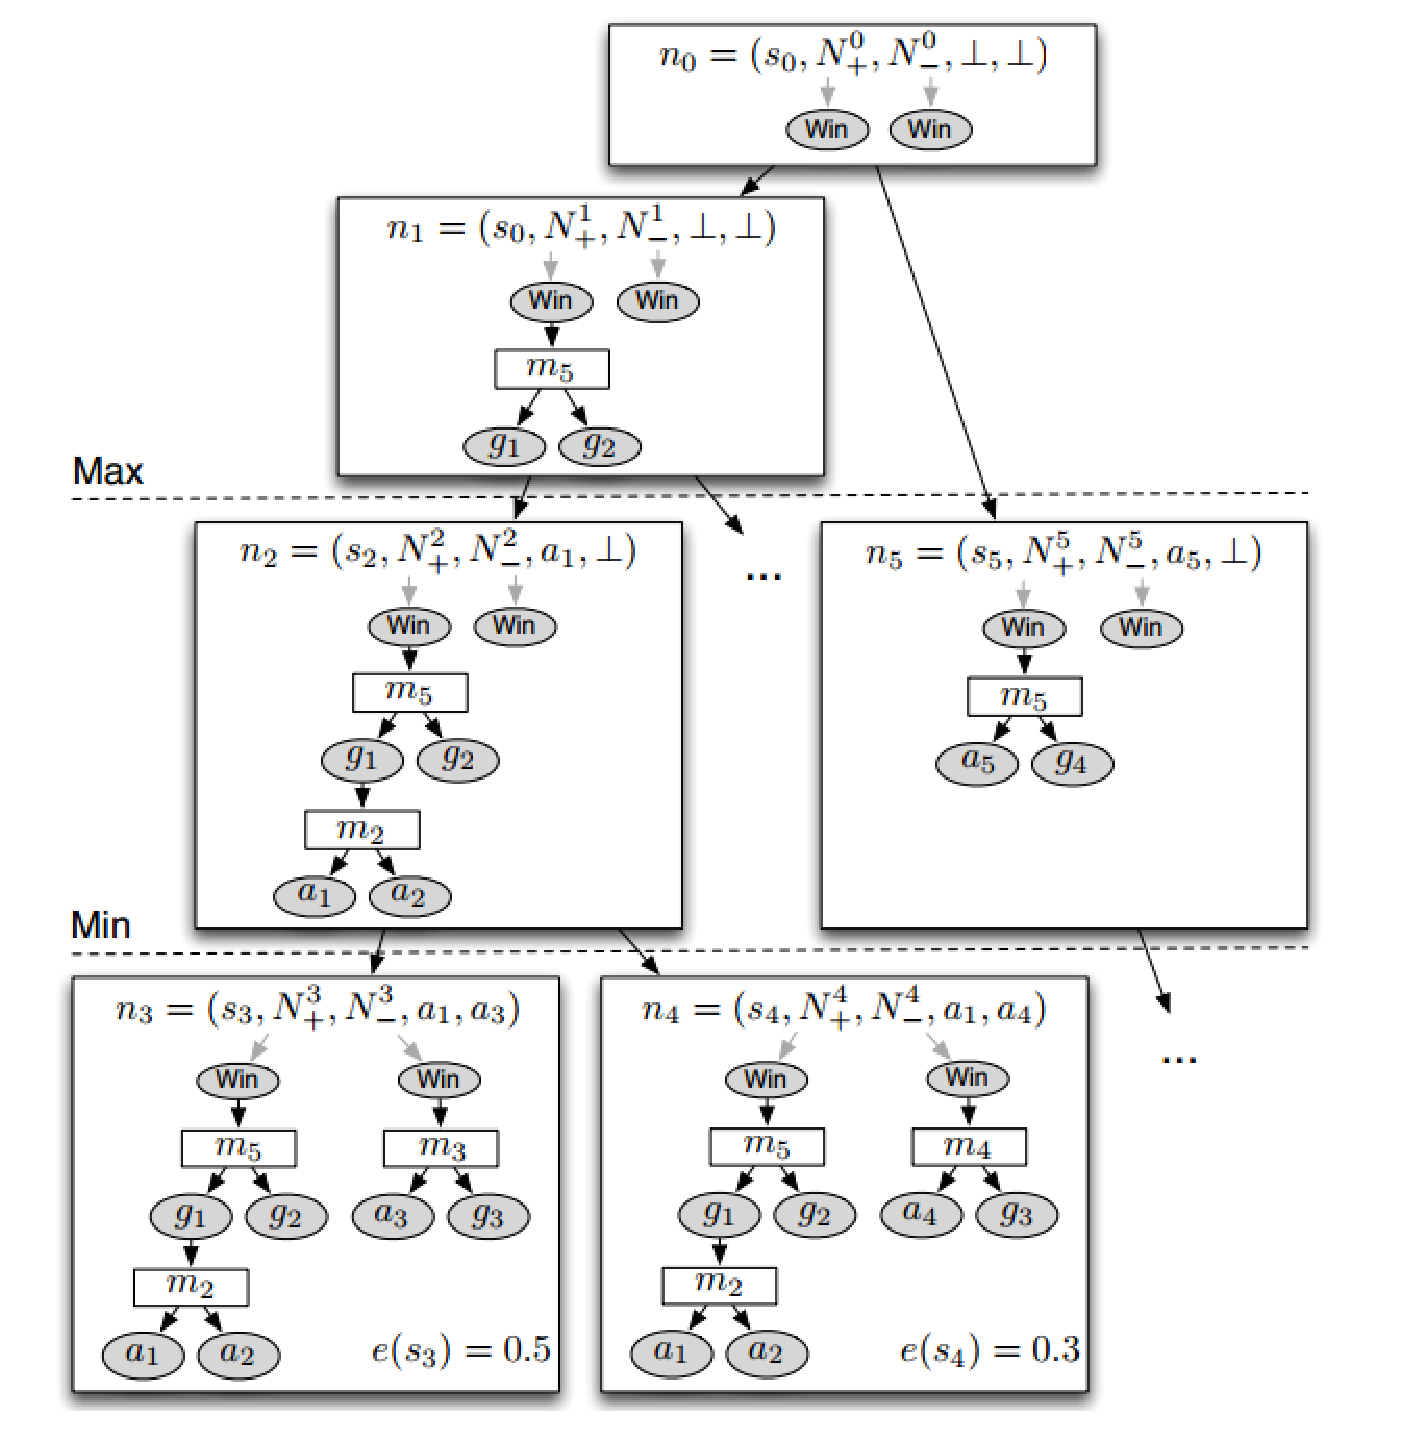
\includegraphics[width=0.35\textwidth]{fig/ahtn.pdf}
	\caption{Arvore gerada pelo algoritmo de AHTN}
	\label{fig:ahtn}
\end{figure} 